\chapter{Equivalence between semistability and $\rho$-semistability}
\section{The equivalent between definitions of semi-stable lattices}
So far we have two distinct definitions of semi-stability. The following theorem asserts that they are equivalent:
\begin{prop}\label{semi-stable-equiv}
    Let $x \in X_n = K \backslash \text{GL}_n(\mathbb{R})$ - the space of unit lattice. Then $x$ is semi-stable if one of the following equaivalent
    conditions holds
    \begin{enumerate}
        \item The bottom of the profile of $x$ is a line connect solely two points: the origin and $(n,0)$.
        \item The degree of instability of $x$ is nonnegative, namely, $\deg_{inst}(x) \ge 0$.
    \end{enumerate}
\end{prop}
\begin{proof}
    \hfill \\
    If we can prove there is a correspondence between
    $\gamma \in \text{GL}_n(\mathbb{Q})/Q_i(\mathbb{Q})$ and a sublattice of rank $i$ of $x$, then we are done.
    We first need a slight reduction - we identified the quotient $\text{GL}_n(\mathbb{Q})/Q_i(\mathbb{Q})$ with
    the quotient $\text{GL}_n(\mathbb{Z})/(Q_i(\mathbb{Q}) \cap \text{GL}_n(\mathbb{Z})) $. Now let $x$ be an arbitrary lattice of rank $n$.

    We will first show the following correspondence
    \[ \text{GL}_n(\mathbb{Z})/(Q_i(\mathbb{Q}) \cap \text{GL}_n(\mathbb{Z})) \longleftrightarrow \left\lbrace \text{ sublattice of rank $i$ of $\mathbb{Z}^n$}\right\rbrace\]
    We define the map from the collection of sublattices of rank $i$ to the cosets space as follows: For any sublattice $M \subset \mathbb{Z}^n$, there exists
    a basis of $M$, denoted by
    \[\left\lbrace v_1,v_2,\ldots, v_i \right\rbrace \]
    we can extend this basis to get a basis of $\mathbb{Z}^n$
    \[\mathfrak{B'} = \left\lbrace v_1,v_2,\ldots, v_n \right\rbrace \]
    Clearly in $\mathbb{Z}^n$ we have the standard basis $\mathfrak{B} = \left\lbrace e_1,e_2,\ldots,e_n\right\rbrace $. Clearly there
    exists a map $\gamma \in \glnz$ such that
    \[\gamma \cdot e_k = v_k \quad \forall k = 1,2,\ldots, n\]
    So we define the map
    \begin{align*}
        \varphi \colon \left\lbrace\text{sublattices of rank $i$ of $\mathbb{Z}^n$}\right\rbrace & \to \text{GL}_n(\mathbb{Z})/(Q_i(\mathbb{Q}) \cap \text{GL}_n(\mathbb{Z})) \\
        M                                                                                        & \mapsto [\gamma]
    \end{align*}
    where $[\gamma]$ denoted the equaivalent class of $\gamma$ in the quotient space. This is a well-defined map. Indeed, Assume that we extend
    the basis $\mathfrak{B'}$ in a different way to get the basis
    \[ \mathfrak{B}_1 = \left\lbrace v_1,\ldots, v_k, v'_{k+1},\ldots,v'_n \right\rbrace\]
    As above, there also exists $\gamma' \in \glnz$ such that
    \[\gamma' e_k = v_k \quad \forall k \le i, \quad \text{ and } \quad \gamma'e_k = v'_k \quad \forall k > i\]
    But this implies that
    \[(\gamma^{-1})\gamma ' \cdot e_k = \gamma^{-1} v_k = e_k \quad \forall k \le i\]
    So in particular, we have $[\gamma] = [\gamma']$. The inverse map is given by
    \[[\gamma] \mapsto \bigoplus_{k=1}^i\mathbb{Z} (\gamma \cdot e_i) = M\]
    This generalizes in the obvious way for lattice $x = g\mathbb{Z}^n$ for some $g \in \text{GL}_n(\mathbb{R})$. Indeed, we just define
    the map
    \begin{align*}
        \phi_g \colon \left\lbrace\text{sublattices of rank $i$ of $g\mathbb{Z}^n$}\right\rbrace & \to \text{GL}_n(\mathbb{Z})/(Q_i(\mathbb{Q}) \cap \text{GL}_n(\mathbb{Z})) \\
        M_g = gM = g \bigoplus_{k=1}^i  \mathbb{Z}v_i                                            & \mapsto [\gamma]
    \end{align*}
    where $\gamma e_k = v_k$ in $\mathbb{Z}^n$ for all $ k \le i$ and $\phi_g^{-1}([\gamma]) = g \bigoplus_{k=1}^i  \mathbb{Z}(\gamma \cdot e_i)$.
\end{proof}\todo{Check the map in the generalization carefully }
\section{Canonical pair and Canonical filtration}
We can further prove that, the equivalence between different notions of semistability
comes from the equivalence between the notion of canonical pair and the bottom of the
profile of a lattice - the canonical filtration. The main result is the following proposition
\begin{prop}\label{cp-equiv}
    Given an $x \in X_n = K\backslash G$. Then $(P,\delta)$ is the canonical pair for $x$ if and only if $P$
    is the stabilizer of the canonical filtration for the lattice $L_x = x\mathbb{Z}^n$.
\end{prop}
Recall that, from theorem \ref{Grayson's criterion} and lemma \ref{canonical-pair}, both canonical
pair and canonical filtration are characterized by two conditions. We will show that these two conditions are equivalent.
Throughout this section, we fix an $x \in X_n$ and the corresponding lattice $L_x= x\mathbb{Z}^n$.
\begin{lemma}\label{increasing-slope}
    The the following conditions are equivalent
    \begin{enumerate}
        \item  $\left\langle \alpha, H_P(x\delta)\right\rangle <0$ for any $\alpha \in \Delta_P$ and for some $\delta \in G_\mathbb{Q}/P_\mathbb{Q}$.
        \item $L_x$ has a chain of vector spaces
              \[\mathcal{F}: 0 = L_0 \subset M_1 \subset M_2 \subset \cdots \subset M_{k-1} \subset M_k = L_x \]
              such that $\mu(M_i/M_{i-1}) <\mu(M_{i+1}/M_i)$ for all $i$. We also attach to the flag
              \[\mathcal{F}\otimes \mathbb{R} \colon L_0 \subset M_1 \otimes \mathbb{R} \subset M_2\otimes \mathbb{R} \subset \cdots \subset M_{k-1}\otimes \mathbb{R} \subset M_k\otimes \mathbb{R} =  \mathbb{R}^n \]
              a rational standard parabolic subgroup $P_\mathbb{Q}$.
    \end{enumerate}
\end{lemma}
\begin{proof}

    We first prove (1) implies (2). Assume that $(P,\delta)$ is the canonical pair for $x$ and
    \[a(x\delta) = \begin{bmatrix}
            a_1    & 0      & \ldots & 0      \\
            0      & a_2    & \ldots & 0      \\
            \vdots & \vdots & \vdots & \vdots \\
            0      & 0      & \ldots & a_n
        \end{bmatrix}\]
    in the Iwasawa decomposition of $x\delta$. We further assume that the standard parabolic
    $P$ in the canonical pair is of type $(n_1,\ldots, n_k)$. Let
    \[d_i = n_1+n_2+\ldots +n_k\]
    Then from the chain of standard lattice
    \[0 \subset \mathbb{Z}^{d_1} \subset \mathbb{Z}^{d_2} \subset \cdots \subset \mathbb{Z}^{d_k}\]
    we obtain a chain of sublattices of $L_x$ as follows
    \[0 \subset M_1 \subset M_2 \subset \cdots \subset M_k\]
    where $$M_i := \bigoplus_{m=1}^{d_i}\mathbb{Z}x\delta \cdot e_m$$.

    Note that for $M_k = x\delta\mathbb{Z}^{d_k} = x\mathbb{Z}^n = L_x$.

    since the volume depend solely on the $A$-coordinate in the Iwasawa decomposition.
    In this way, it is immediate that the volume of the sublattice $M_i$ is
    \[\vol(M_i) = a_1a_2\cdots a_i,\]
    \begin{figure}[hbt]
        \centering
        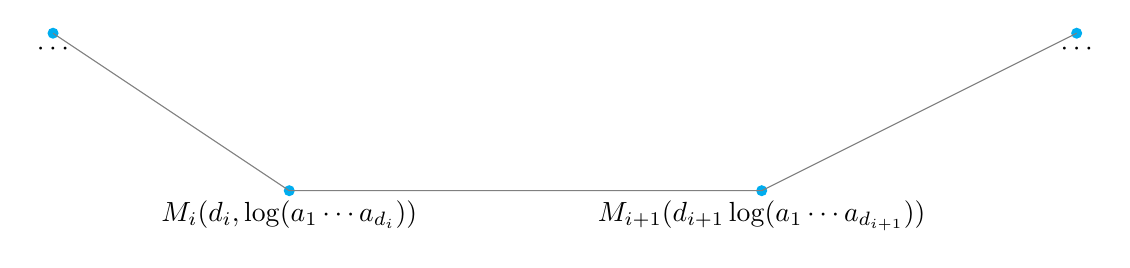
\begin{tikzpicture}
            % Coordinates
            \coordinate (D) at (2,-2);
            \coordinate (F) at (4,2.5);
            \coordinate (E) at (8,-2);
            \coordinate (G) at (-1,0);
            \coordinate (H) at (12,0);
            % Labels
            \node at (G) [below] {$\cdots$};
            \node at (D) [below] {$M_i(d_i,\log(a_1\cdots a_{d_i}))$};
            \node at (E) [below ] {$M_{i+1}(d_{i+1}\log(a_1\cdots a_{d_{i+1}}))$};
            \node at (H) [below ] {$\cdots$};
            % Points
            \fill[cyan] (E) circle (2pt);
            \fill[cyan] (D) circle (2pt);
            \fill[cyan] (G) circle (2pt);
            \fill[cyan] (H) circle (2pt);

            % draw additional lines
            \draw[gray] (G) -- (D)-- (E) -- (H);
        \end{tikzpicture}
        \caption{}
        \label{figureproof}
    \end{figure}



    We will show that
    \[H_P(x\delta ) =m_1\lambda^\vee_{d_1}+m_2\lambda^\vee_{d_2}+\ldots+m_k\lambda^\vee_{d_k}\]
    where
    \[m_i = \dfrac{\log(a_{d_{i-1}}\cdots a_{d_i})}{n_i}-\dfrac{\log(a_{d_i+1}\cdots a_{d_{i+1}})}{n_{i+1}}\]
    If we can prove this, we are done, as
    \[ \mu(M_i/M_{i-1})-\mu(M_{i+1}/M_i)= m_i =\left\langle\alpha_{d_i},H_P(x\delta) \right\rangle < 0\]
    Hence we recover the second condition in Grayson's criterion, namely, $\mu(M_i/M_{i-1}) \le \mu(M_{i+1}/M_i)$ for all $1 \le i \le k-1$.

    To prove this, we first note that
    \begin{align*}
        H_B(x\delta) & =  \log(a_1)\alpha_i^\vee+\log(a_1a_2)\alpha_2^\vee+\ldots \log(a_1a_2\cdots a_{n-1})\alpha_{n-1}^\vee             \\
                     & = \log\left(\dfrac{a_1}{a_2}\right)\lambda_1^\vee+\ldots + \log\left(\dfrac{a_{n-1}}{a_n}\right)\lambda_{n-1}^\vee
    \end{align*}
    To compute $H_P(x\delta)$, we will use the Lemma \ref{H_P-decomp} to get
    \[H_B =H_P + H_{\star B}\]
    and Lemma \ref{coeff-H(J)} to compute $H_{\star B}$ explicitly. Since $P$ is a standard parabolic
    subgroup, we have $P=P_J$ and thus
    \[H_{\star B}(x\delta) = \sum_{i \notin J} \log\left(\dfrac{a_i}{a_{i+1}}\right)\lambda_{i,J}^\vee\]
    We want to write $\lambda_{i,J}^\vee$ as linear combination of $\alpha_j^\vee$'s. To do this, we use
    the theorem \ref{cartaininverse}.

    Note that we can write $H_P(x\delta)$ in two ways
    \begin{align*}
        H_P(x\delta) & = H_B(x\delta) - H_{\star B}(x\delta)                                     \\
                     & = \sum_{j=1}^{n-1}t_j\alpha_j^\vee                                        \\
                     & =m_1\lambda^\vee_{d_1}+m_2\lambda^\vee_{d_2}+\ldots+m_k\lambda^\vee_{d_k}
    \end{align*}
    Then by \ref{weight-root-comb}, we must have
    \[m_i = 2t_{d_i}-t_{d_{i}-1}+t_{d_i+1}\]
    for $1<i<k$. To compute $t_{d_i}$, we find the coefficient of $\alpha_{d_i}^\vee$. But this
    is just the coefficient of $\alpha_{d_i}^\vee$ in the linear combination of $H_B(x\delta)$. Thus
    \[t_{d_i} = \log(a_1\cdots a_{d_i})  \]
    The value of $t_{d_i-1}$ and $t_{d_i+1}$ is slightly more complicated. For $t_{d_i-1}$, it is the difference between
    the coefficient of $\alpha_{d_i-1}^\vee$ in $H_B(x\delta)$ and that of $\alpha_{d_i-1}^\vee$ in $H_{\star B}(x\delta)$.
    By lemma \ref{cartaininverse}, we have
    \begin{align*}
        \sum_{s=p}^q\log\left(\dfrac{a_s}{a_{s+1}}\right)\lambda^\vee_s
         & =\begin{bmatrix}
                \log\left(\dfrac{a_p}{a_{p+1}}\right) & \cdots & \log\left(\dfrac{a_q}{a_{q+1}}\right)
            \end{bmatrix}
        \begin{bmatrix}
            \lambda_p^\vee \\
            \vdots         \\
            \lambda_q^\vee
        \end{bmatrix}                                                                                                                                     \\
         & =\begin{bmatrix}
                \log\left(\dfrac{a_p}{a_{p+1}}\right) & \cdots & \log\left(\dfrac{a_q}{a_{q+1}}\right)
            \end{bmatrix}  A^{-1} \begin{bmatrix}
                                      \lambda_p^\vee \\
                                      \vdots         \\
                                      \lambda_q^\vee
                                  \end{bmatrix}
    \end{align*}
    So the coefficient of $\alpha_{d_i-1}^\vee$ in $H_{\star B} (x\delta)$ is
    \[\sum_{u=1}^{n_i-1}\log\left(\dfrac{a_{d_{i-1}+u}}{a_{d_{i-1}+u+1}}\right)\left(\min\{u,n_i-1\}-\dfrac{u(n_i-1)}{n_i}\right)=\sum_{u=1}^{n_i-1}\log\left(\dfrac{a_{d_{i-1}+u}}{a_{d_{i-1}+u+1}}\right)\dfrac{u}{n_i}\]
    Argue similarly, we can also find the value of $t_{d_i+1}$. Overall, we have
    \begin{align*}
        \begin{cases}
            \displaystyle  t_{d_i-1} = \log(a_1\cdots a_{d_i-1})-\sum_{u=1}^{n_i-1}\log\left(\dfrac{a_{d_{i-1}+u}}{a_{d_{i-1}+u+1}}\right)\dfrac{u}{n_i}                  \\
            \displaystyle t_{d_i+1}= \log(a_1\cdots a_{d_i+1})-\sum_{u=1}^{n_{i+1}-1}\log\left(\dfrac{a_{d_{i}+u}}{a_{d_{i}+u+1}}\right)\left(1-\dfrac{u}{n_{i+1}}\right) \\
        \end{cases}
    \end{align*}
    which simplify to $m_i = \dfrac{\log(a_{d_{i-1}}\cdots a_{d_i})}{n_i}-\dfrac{\log(a_{d_i+1}\cdots a_{d_{i+1}})}{n_{i+1}}$ as desired.
    The cases $i=1,k$  can be verified similarly.

    Conversely, assume that we have a a chain
    \[\mathcal{F}: 0 = L_0 \subset M_1 \subset M_2 \subset \cdots \subset M_{k-1} \subset M_k = L_x \]
    Then multiplying by $x^{-1}$ on the left gives a chain of lattices in $\mathbb{Z}^n$.
    \[\mathcal{F}: 0 = L_0 \subset N_1 \subset N_2 \subset \cdots \subset N_{k-1} \subset N_k ^n= \mathbb{Z} \]
    where $N_i:= x^{-1}M_i$. Let us denote $n_i:=\rk(N_i)$. Then there exists an ordered
    basis for the standard lattice $\mathbb{Z}^n$
    \[\mathcal{B} = \left\lbrace v_1,v_2,\ldots, v_n \right\rbrace\]
    such that $\{v_1,\ldots,v_{n_i}\}$ is the basis for the lattice $N_i$. We clearly can find an element
    $\delta \in \glnz$ such that $\delta\cdot v_i = e_i$. Repeat the argument in Theorem \ref{semi-stable-equiv}, we can see that
    $\delta\eta$ stabilizes the flag $\mathcal{F}$. So it does not change anything if we consider the coset $\delta P_\mathbb{Q}$.
    Consider the element $x\delta$ for $\delta \in G_\mathbb{Q}/P_\mathbb{Q}$ and do the same computation for
    $x\delta$ as in the $1 \Rightarrow 2$ part, we can see that
    \[0 > \mu(M_i/M_{i-1})-\mu(M_{i+1}/M_i)= m_i =\left\langle\alpha_{d_i},H_P(x\delta) \right\rangle\]
    Thus the lemma is proved.
\end{proof}
\begin{remark}
    From the proof the lemma \ref{increasing-slope}, we explicitly construct an equivalence
    \[xG_\mathbb{Q}/P_\mathbb{Q} \longleftrightarrow \{\mbox{ flag of sublattices of $x\mathbb{Z}^n$ of the same type of partition type of $P$}\}\]

\end{remark}
\begin{lemma}\label{ss-slope}
    Fixed the notations as in lemma \ref{increasing-slope}, the following conditions are equivalent
    \begin{enumerate}
        \item $M_i/M_{i-1}$ is semistable for all $i$, where the flag
              \[\mathcal{F}: 0  \subset M_1 \subset M_2 \subset \cdots \subset M_{k-1} \subset M_k = L_x \]
              corresponds to $x\delta$.
        \item $x\delta$ is $P-$semistability for some $\delta \in G_\mathbb{Q}/P_\mathbb{Q}$.
    \end{enumerate}
\end{lemma}
\begin{proof}
    \hfill \\
    We prove $1 \Rightarrow 2$ by contradiction. Assume not, then there exists a maximal
    parabolic subgroup $Q \subset P$ and an $\eta \in P/Q$ such that
    \[\left\langle \rho_Q^P, H_Q(x\delta\eta) \right\rangle < 0\]
    by lemma \ref{ss-equiv}. We assume that $P$ is a standard parabolic subgroup of type $(n_1,n_2,\ldots,n_k)$. Then
    Q must be of the type $(n_1,\ldots, n_{i,1},n_{i,2},\ldots,n_k)$ where $n_{i,1}+n_{i,2} = n_i$
    for some $1 \le i \le k$.  Argue as in lemma \ref{increasing-slope}, we obtain a chain of sublattices of $L_x$
    \[0 \subset M_{1} \subset \cdots M_{{i-1}} \subset M'\subset M_{{i+1}} \subset \cdots \subset M_{k} = L_x\]
    where $\rk(M_j)=d_j$ for $j \ne i$ and $\rk(M') = d_{i-1}+n_{i,1} =r$.

    Using the same computation as in lemma \ref{increasing-slope}, it can be seen that
    \[0 > \left\langle\rho_Q^P, H_Q(x\delta\eta)\right\rangle = c \left\langle \alpha_r,H_Q(x\delta\eta) \right\rangle= c\cdot\left(\mu(M'/M_{i-1})-\mu(M_{i+1}/M')\right) \]
    In particular
    \[\mu(M'/M_{i-1})-\mu(M_{i+1}/M') < 0 \Leftrightarrow \mu(M'/M_{i-1})<\mu(M_{i+1}/M')\]
    But this contradicts the fact that $M_i/M_{i-1}$ is a semistable for all $i$, i.e.
    there are no sublattices $M'$ such that $\ell(M')$ lies below the line connectings
    $\ell(M_i)$ and $\ell(M_{i-1})$ for all $i$.
    \begin{figure}[hbt]
        \centering
        \begin{tikzpicture}
            % Coordinates
            \coordinate (D) at (2,-2);
            \coordinate (F) at (4,2.5);
            \coordinate (A) at (6,-4);
            \coordinate (E) at (8,-3);
            \coordinate (G) at (-1,0);
            \coordinate (H) at (12,-1);
            % Labels
            \node at (A) [below] {$\ell(M')$};
            \node at (D) [below] {$\ell(M_{i-1})$};
            \node at (E) [below ] {$\ell(M_{i})$};
            % Points
            \fill[cyan] (E) circle (2pt);
            \fill[cyan] (D) circle (2pt);
            \fill[cyan] (A) circle (2pt);
            \fill[cyan] (H) circle (2pt);
            \fill [cyan] (G) circle (2pt);
            % draw additional lines
            \draw[thick,black] (G) -- (D)-- (E) -- (H);
            \draw[red] (D) -- (A) -- (E);
        \end{tikzpicture}
        \caption{}
        \label{figureproof}
    \end{figure}

    Conversely, to prove $2 \Rightarrow 1$, we also prove by contradiction.
    Assume that $M_i/M_{i-1}$ is unstable for some index $i$. Then there exists
    a flag
    \[ 0 \subset M^\ast \subset M_i/M_{i-1}\]
    such that $\mu(M^\ast) <\mu(M_i/M_{i-1})$. Let $M':= M^\ast \oplus M_{i-1}$, then
    $M'$ is a sublattice of $M_i$ containing $M_{i-1}$ such that
    \[\mu(M'/M_{i-1}) < \mu (M_i/M_{i-1}) = \dfrac{rk (M'/M_{i-1})}{\rk(M_i/M_{i-1})}\mu(M'/M_{i-1})+\dfrac{rk (M_i/M')}{\rk(M_i/M_{i-1})}\mu(M_i/M') \]
    which implies that
    \[\mu(M'/M_{i-1})<\mu(M_i/M')\]
    Since the chain
    \[0 \subset M_{1} \subset \cdots M_{{i-1}} \subset M'\subset M_{{i+1}} \subset \cdots \subset M_{k} = L_x\]
    is a refinement of the flag $\mathcal{F}$, this gives rise to a pair $(Q,\delta')$ where $Q\subset P$
    is a maximal standard parabolic subgroup of $P$ and $\delta'P=\delta P$. But then again we have
    \[ \left\langle\rho_Q^P, H_Q(x\delta\eta)\right\rangle = c \left\langle \alpha_r,H_Q(x\delta\eta) \right\rangle= c\cdot\left(\mu(M'/M_{i-1})-\mu(M_{i+1}/M')\right)<0 \]
    which is a contradiction.
\end{proof}
Combinining Lemmas \ref{ss-slope} and \ref{increasing-slope}, we get a proof
for proposotion \ref{cp-equiv} as follows
\begin{proof}
    Assume that $(P,\delta)$ is a canonical pair for $x$, then there exists a
    flag
    \[\mathcal{F}: 0 = L_0 \subset M_1 \subset M_2 \subset \cdots \subset M_{k-1} \subset M_k = L_x \]
    that corresponds to $x\delta$ and admits $P_\mathbb{Q}$ as its stabilizer. Lemmas \ref{increasing-slope}
    and \ref{ss-slope} guarantees that this flag satisfies two condition in Grayson's criterion \ref{Grayson's criterion}, thus
    $\mathcal{F}$ is the canonical filtration. Conversely, let $\mathcal{F}$ be the canonical
    filtration for $x$ and denote $Q$ the stabilizer of $\mathcal{F}$. If $(P,\delta)$ is the canonical pair, it also gives
    rise to a canonical flag $\mathcal{F'}$. Theorem \ref{filtration} ensures that the canonical filtration is unique, thus
    $\mathcal{F} \equiv \mathcal{F'}$. Consenquently, we must have $Q=P$.
\end{proof}
\begin{remark}
    The construction above also shows that the canonical pair, must be unique and determined by the canonical filtration.
\end{remark}